\subsection*{A:}
\label{sub:a_}

The stability analysis of the jacobi solver did not converge to the
analytical value for increasing $\rhomax$, as this increased the step size
and caused reduced precision. For $N=200$, a $\rhomax$ of $\approx 5$ was
found ideal for the third wavefunction in the non interacting harmonic
oscillator. Then setting $\rhomax$ equal to 


\begin{figure}[htpb]
    \centering
    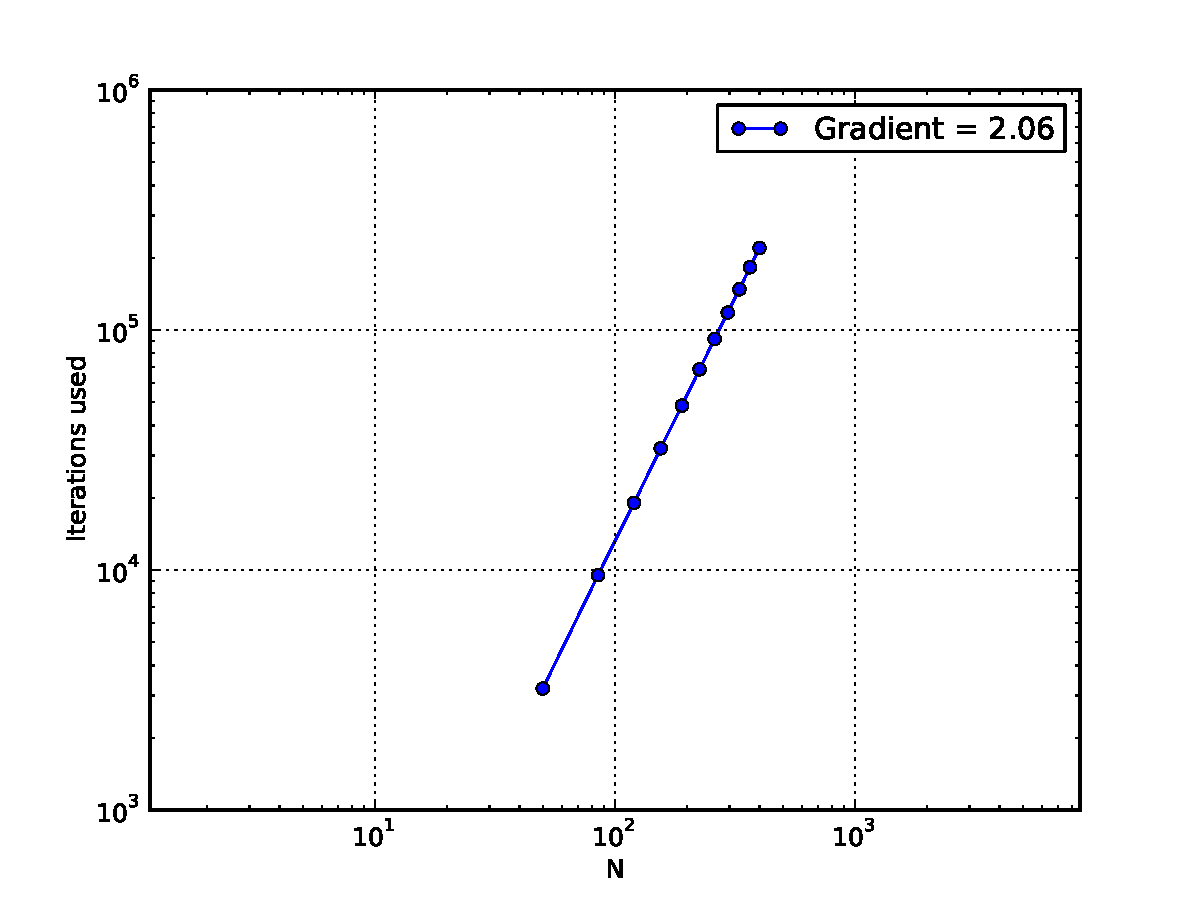
\includegraphics[width=0.8\linewidth]{iterations.pdf}
    \caption{Iterations of jacobi rotate vs N}
    \label{fig:iterations}
\end{figure}

\begin{figure}[htpb]
    \centering
    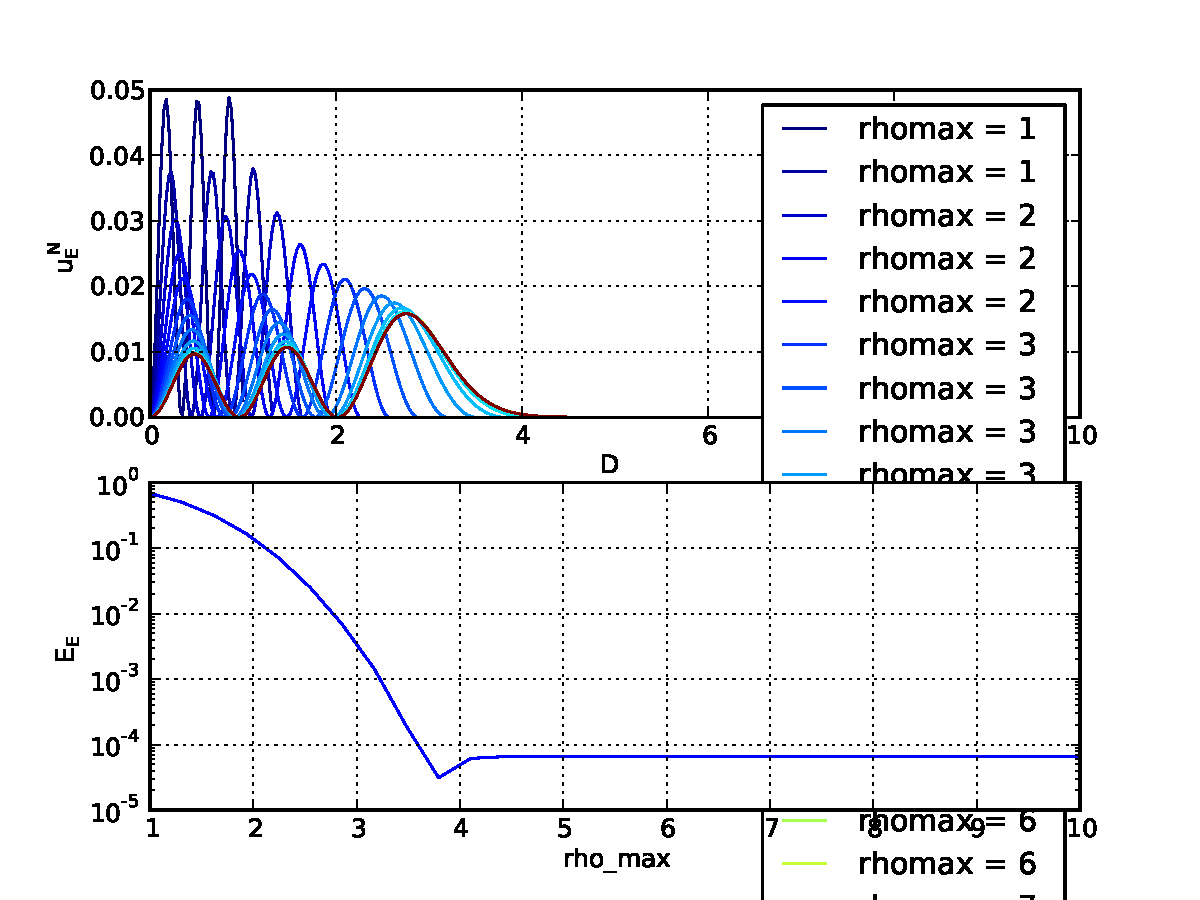
\includegraphics[width=0.8\linewidth]{rhoMaxAnalysis.pdf}
    \caption{RhoMaxAnalysis}
    \label{fig:rhoMaxAnalysis}
\end{figure}

\begin{figure}[htpb]
    \centering
    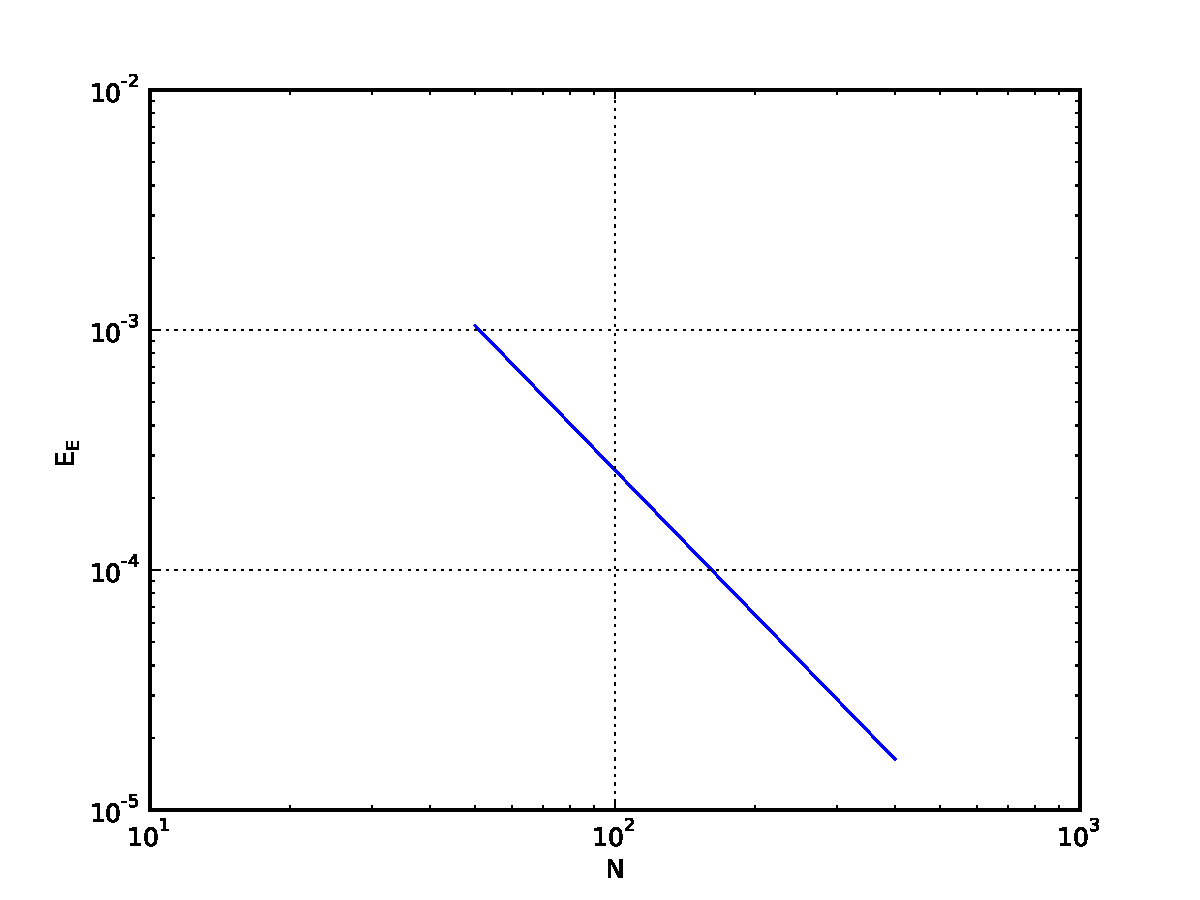
\includegraphics[width=0.8\linewidth]{dimAnalysis.pdf}
    \caption{DimAnalysis}
    \label{fig:dimAnalysis}
\end{figure}

\begin{figure}[htpb]
    \centering
    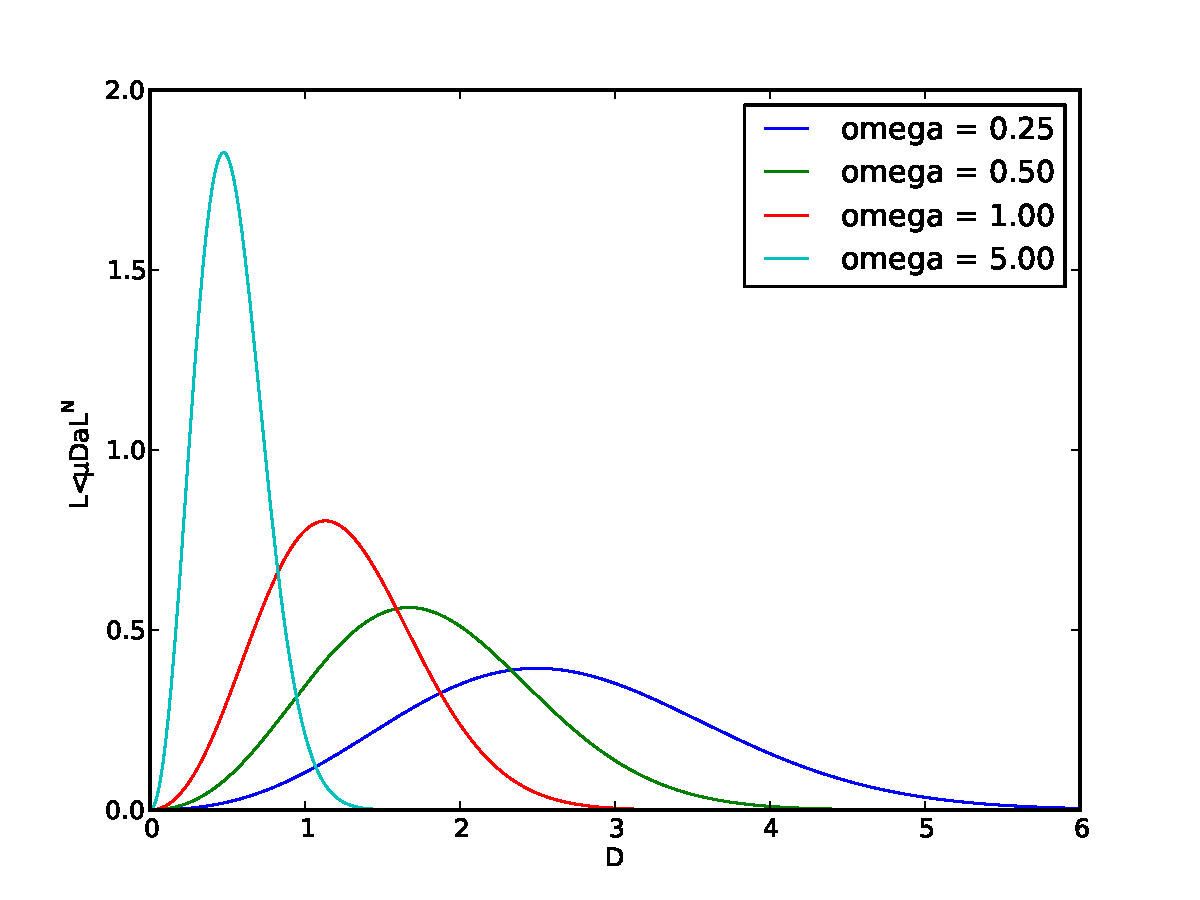
\includegraphics[width=0.8\linewidth]{waveFunc.pdf}
    \caption{WaveFunc }
    \label{fig:waveFunc}
\end{figure}



\begin{equation}
    
\end{equation}
